\documentclass[tikz,border=3pt]{standalone}
\pdfinfoomitdate=1
\pdftrailerid{}
\pdfsuppressptexinfo=15
\usepackage{amsmath,amssymb}
\usepackage{braket}
\usetikzlibrary{arrows.meta,backgrounds,fit,positioning}
\definecolor{sourceblue}{RGB}{218,235,248}
\definecolor{targetgreen}{RGB}{222,242,229}
\definecolor{stageviolet}{RGB}{239,232,248}
\begin{document}
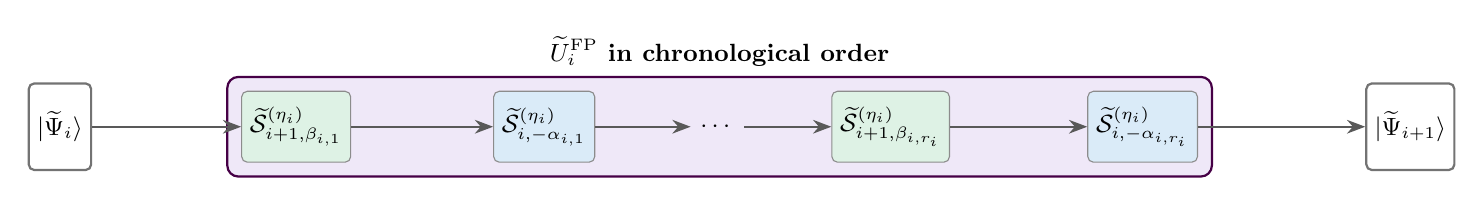
\begin{tikzpicture}[
  >=Stealth,
  font=\small,
  state/.style={draw=black!55,thick,rounded corners=2pt,fill=white,
    minimum height=11mm,align=center,inner sep=3pt},
  phase/.style={draw=black!45,rounded corners=2pt,minimum height=9mm,
    align=center,inner sep=3pt},
  flow/.style={->,thick,draw=black!65},
]
\node[state] (input) at (0,0) {$\ket{\widetilde\Psi_i}$};
\node[phase,fill=targetgreen] (t1) at (3.0,0)
  {$\widetilde{\mathcal S}_{i+1,\beta_{i,1}}^{(\eta_i)}$};
\node[phase,fill=sourceblue] (s1) at (6.15,0)
  {$\widetilde{\mathcal S}_{i,-\alpha_{i,1}}^{(\eta_i)}$};
\node (dots) at (8.35,0) {$\cdots$};
\node[phase,fill=targetgreen] (tr) at (10.55,0)
  {$\widetilde{\mathcal S}_{i+1,\beta_{i,r_i}}^{(\eta_i)}$};
\node[phase,fill=sourceblue] (sr) at (13.75,0)
  {$\widetilde{\mathcal S}_{i,-\alpha_{i,r_i}}^{(\eta_i)}$};
\node[state] (output) at (17.15,0)
  {$\ket{\widetilde\Psi_{i+1}}$};

\draw[flow] (input) -- (t1);
\draw[flow] (t1) -- (s1);
\draw[flow] (s1) -- (dots);
\draw[flow] (dots) -- (tr);
\draw[flow] (tr) -- (sr);
\draw[flow] (sr) -- (output);

\begin{scope}[on background layer]
\node[draw=violet!55!black,thick,rounded corners=4pt,fill=stageviolet,
  fit=(t1)(s1)(dots)(tr)(sr),inner sep=5pt,
  label={[font=\bfseries\small]above:
  $\widetilde U_i^{\mathrm{FP}}$ in chronological order}] (stage) {};
\end{scope}

\end{tikzpicture}
\end{document}
